Eine flache Platte ist um eine feste Achse durch D drehbar, die senkrecht zur Platte steht. Vier Kräfte wirken auf sie, gezeichnet auf einem Gitter aus Kästchen von \SI{10}{\cm}:
\begin{itemize}
 \item $F_1 = \FaO$ schräg nach rechts oben mit der Steigung $3:4$ (4 Kästchen nach rechts, 3 nach oben), Angriffspunkt 2 Kästchen rechts von und 1 Kästchen über D,
 \item $F_2 = \FbO$ nach links, Angriffspunkt 3 Kästchen links von D,
 \item $F_3 = \FcO$ nach oben, Angriffspunkt 2 Kästchen links von und 2 Kästchen über D,
 \item $F_4 = \FdO$ nach links, Angriffspunkt 1 Kästchen rechts von und 4 Kästchen unter D.
\end{itemize}
\begin{center}
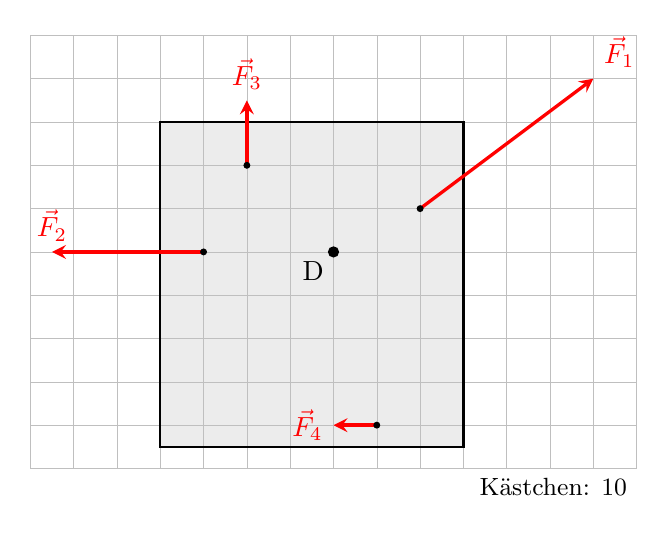
\begin{tikzpicture}[scale=0.55, >=stealth]
 \fill[gray!15] (-4,-4.5) -- (3,-4.5) -- (3,3) -- (-4,3) -- cycle;
 \draw[gray!50, very thin] (-7,-5) grid (7,5);
 \draw[thick] (-4,-4.5) -- (3,-4.5) -- (3,3) -- (-4,3) -- cycle;
 \fill (0,0) circle (0.13) node[below left] {D};
 \draw[->, very thick, red] (2,1) -- (6,4) node[above right] {$\vec F_1$};
 \draw[->, very thick, red] (-3,0) -- (-6.5,0) node[above] {$\vec F_2$};
 \draw[->, very thick, red] (-2,2) -- (-2,3.5) node[above] {$\vec F_3$};
 \draw[->, very thick, red] (1,-4) -- (0,-4) node[left] {$\vec F_4$};
 \foreach \p in {(2,1),(-3,0),(-2,2),(1,-4)} \fill \p circle (0.08);
 \node[below left] at (7,-5) {\small Kästchen: \SI{10}{\cm}};
\end{tikzpicture}
\end{center}

\begin{abcliste}
\abc
Bestimme das Drehmoment jeder Kraft bezüglich D und ihren Drehsinn. Zerlege dazu $F_1$ in eine waagrechte und eine senkrechte Komponente.

\abc
Ordne die vier Drehmomente nach ihrem Betrag, das kleinste zuerst. Hat die grösste Kraft das grösste Drehmoment?

\abc
Wie lang ist der Hebelarm von $F_1$? Vergleiche ihn mit dem Abstand von D zum Angriffspunkt.

\abc
Alle vier Kräfte wirken gleichzeitig. In welchem Drehsinn beginnt sich die Platte zu drehen?
\end{abcliste}
